\section{Introduction}
\label{network:ntlm:authentication}
LM and  NTLM here are the hash names, and NTLMv1 and NTLMv2 are authentication  protocols that utilize the LM or NT hash. Below is a quick comparison  between these hashes and protocols, which shows us that, while not  perfect by any means, Kerberos is often the authentication protocol of  choice wherever possible. It is essential to understand the difference  between the hash types and the protocols that use them.

\begin{tabular}{|l|l|l|l|l|}
 \hline \hline
 Hash     & Crypto    & Mutual & Msg Type & Trusted  \\
 Protocol & technique &  Authn &          & 3d Party \\
 \hline \hline
 NTLM & Sym  & No & Rnd nbr & DC \\
 NTLMv1 & Sym  & No & MD4 hash, rnd nbr & DC \\
 NTLMv2 & Sym  & No & MD4 hash, rnd nbr & DC \\
 Kerberos & Sym \& Asym & Yes & Encrypted ticket using DES, MD5 & DC, KDC \\
 \hline \hline
\end{tabular}

\subsection{Hashes}
\subsubsection{LM}

LAN Manager (LM) hashes are the oldest password storage Windows operating system. Due to significant security weaknesses in the hashing  algorithm it has been turned off by default since  Windows Vista/Server 2008. However, it is still common to encounter,  especially in large environments where older systems are still used.  Passwords using LM are limited to a maximum of 14  characters. Passwords are not case sensitive and are converted to  uppercase before generating the hashed value, limiting the keyspace to a  total of 69 characters making it relatively easy to crack these hashes  using a tool such as Hashcat.

An LM hash takes the form of \verb+299bd128c1101fd6+.

\subsubsection{NTHash (NTLM)}

These hashes are stored locally in the SAM database or the \gls{win:NTDS.DIT}
database file on a Domain Controller. The protocol has two hashed  password
values to choose from to perform authentication: the LM hash (as discussed
above) and the NT hash, which is the MD4 hash of the little-endian UTF-16 value
of the password.

Even though they are considerably stronger than LM hashes (supporting the entire Unicode character set of 65,536 characters), they can still  be brute-forced offline relatively quickly using a tool such as Hashcat. NTLM is also vulnerable to the  pass-the-hash attack.

An NTLM hash looks like this:

\begin{verbatim}
Rachel:500:aad3c435b514a4eeaad3b935b51304fe:e46b9e548fa0d122de7f59fb6d48eaa2:::
\end{verbatim}

Looking at the hash above, we can break the NTLM hash down into its individual parts:
\begin{itemize}
    \item  \verb+Rachel+ is the username
    \item  \verb+500+ is the Relative Identifier (RID). 500 is the known RID for the administrator account
    \item  \verb+aad3c435b514a4eeaad3b935b51304fe+ is the LM hash and, if LM hashes are disabled on the system, can not be used for anything
    \item  \verb+e46b9e548fa0d122de7f59fb6d48eaa2+ is the NT hash. This hash can either be cracked offline or used for a pass-the-hash attack.
\end{itemize}

\subsection{Protocols}

NT Lan Manager (NTLM/MS-NLMP) is the name of a family of security protocols (LM, NTLMv1, and NTLMv2) used by application protocols to authenticate remote users and optionally provide session security when requested by the application.

The NTLM security protocols are all embedded protocols, meaning that although NTLM has messages and a state machine like other protocols, it does not have a network protocol stack layer. This nature of NTLM allows any protocol with a defined layer in the network stack (such as SMB, HTTP(S), and LDAP(S)) to utilize it.

NTLM is a challenge-response protocol that uses nonces, pseudo-random numbers generated for one-time use, as a defensive mechanism against replaying attacks.

Each protocol has two variants, connection-oriented and connectionless.

\begin{itemize}
    \item 
        Security Support Provider Interface (SSPI) is an API that allows connected applications to call one of several security providers to establish authenticated connections and to exchange data securely over those connections.
    \item  
        A security support provider (SSP) is a dynamic-link library (DLL) responsible for implementing the SSPI by exposing one or more security packages to applications; each security package provides mappings between an application's SSPI function calls and an actual security model's functions. 
    \item 
        NTLM SSP (\verb+%Windir%\System32\msv1_0.dll+) is a binary messaging protocol utilized by SSPI to facilitate NTLM challenge-response authentication and to negotiate options for integrity and confidentiality
\end{itemize}

Both domain-joined and workgroup computers can utilize NTLM for authentication

always keep in mind the following:
\begin{itemize}
    \item 
        The NTLM version used on hosts, whether NTLMv1 or NTLMv2, is \href{https://learn.microsoft.com/en-us/windows/security/threat-protection/security-policy-settings/network-security-lan-manager-authentication-level}{configured out-of-band} before authentication.
    \item
        Using a secure mechanism, the client and server/DC share a secret key (the user's password's hash) before authentication.
    \item
        Neither plaintext credentials nor the shared secret key are sent over the wire.
\end{itemize}


\subsubsection{Authentication Workflow}

NT LAN Manager (NTLM) hashes are used on modern Windows  systems. It is a
challenge-response authentication protocol and uses  three messages to
authenticate: 
\begin{enumerate}
    \item {\bf Negotiate} a client first sends a
        \href{https://docs.microsoft.com/en-us/openspecs/windows_protocols/ms-nlmp/b34032e5-3aae-4bc6-84c3-c6d80eadf7f2}{NEGOTIATE\_MESSAGE}+ to the server
    \item {\bf Challenge} the server sends a challenge to the client. This is
        nothing more than a 64-bit random value that changes with each
        authentication request
        (\href{https://docs.microsoft.com/en-us/openspecs/windows_protocols/ms-nlmp/801a4681-8809-4be9-ab0d-61dcfe762786}{CHALLENGE\_MESSAGE}).
    \item {\bf Response} The client encrypts the previously received challenge
        using a hashed version of its password as the key, and returns this
        encrypted version to the server, along with its username and possibly
        its domain
        (\href{https://docs.microsoft.com/en-us/openspecs/windows_protocols/ms-nlmp/033d32cc-88f9-4483-9bf2-b273055038ce}{AUTHENTICATE\_MESSAGE})
\end{enumerate}

\begin{figure}[!ht]
  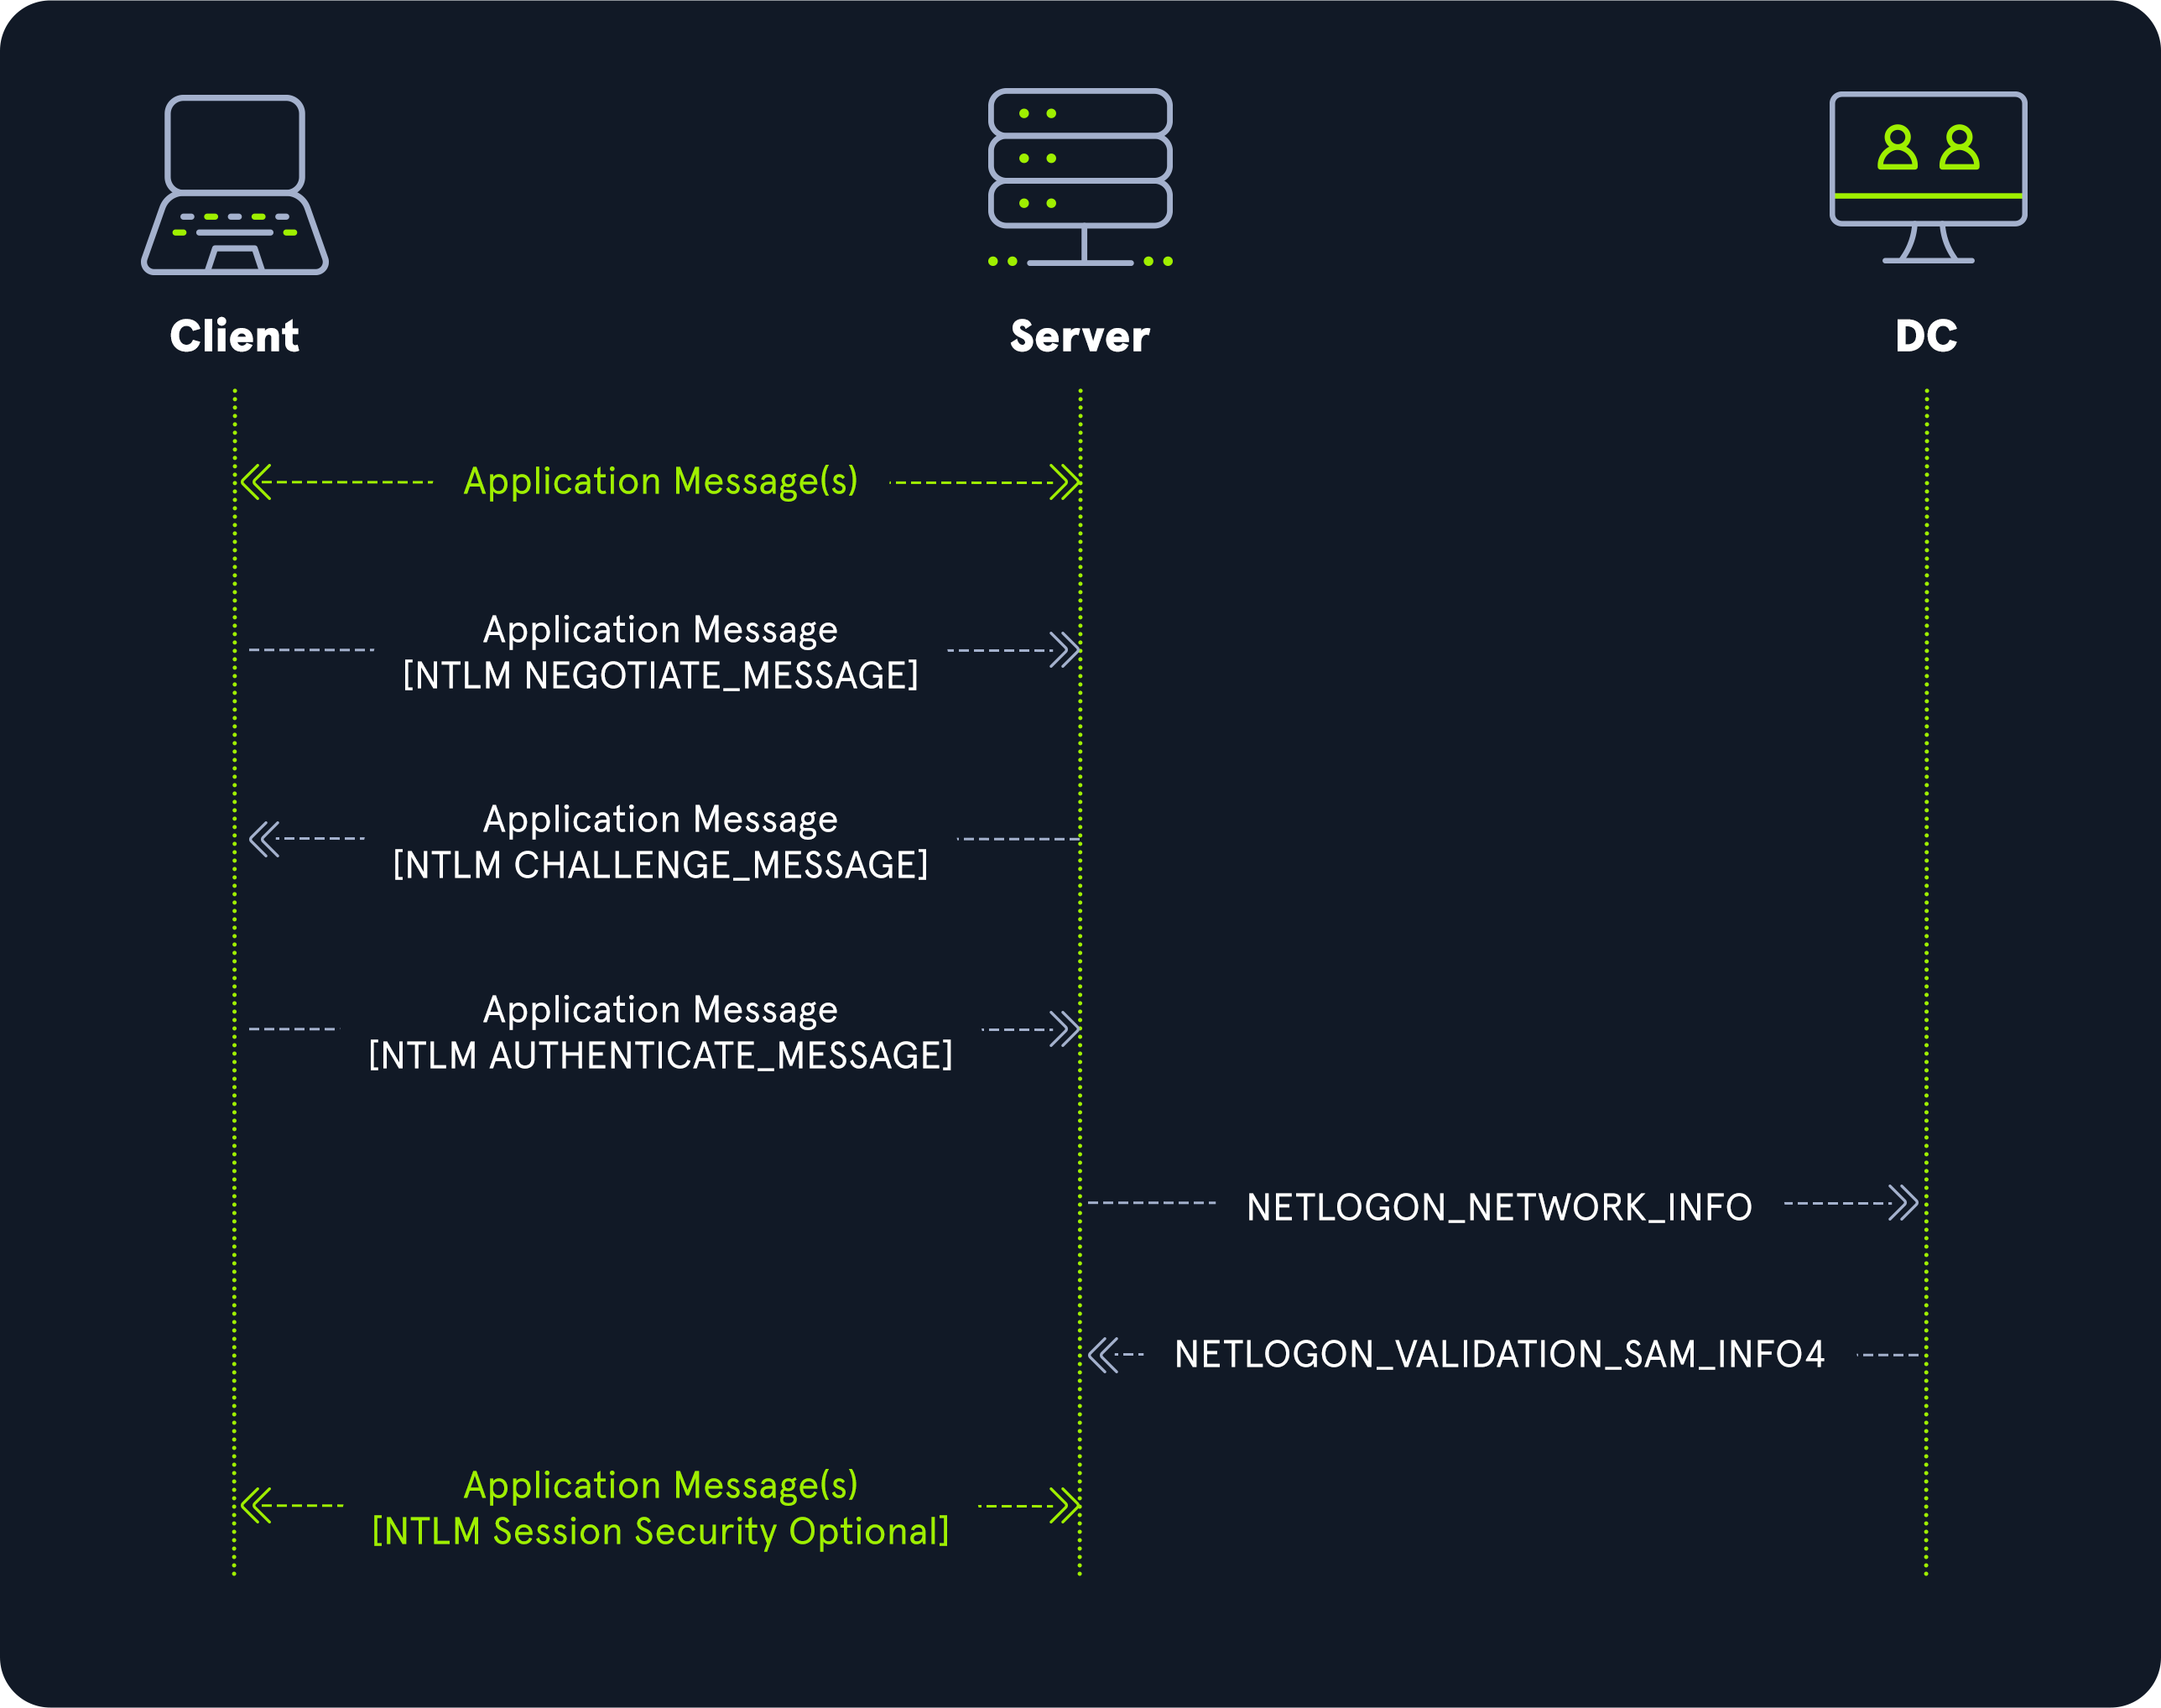
\includegraphics[width=\linewidth]{network/ntlm/images/Domain-joined_Computers_NTLM_Authentication.png}
  \caption{Domain joined NTLM protocol}
  \label{fig:domain-ntlm-protocol}
\end{figure}

\begin{figure}[!ht]
  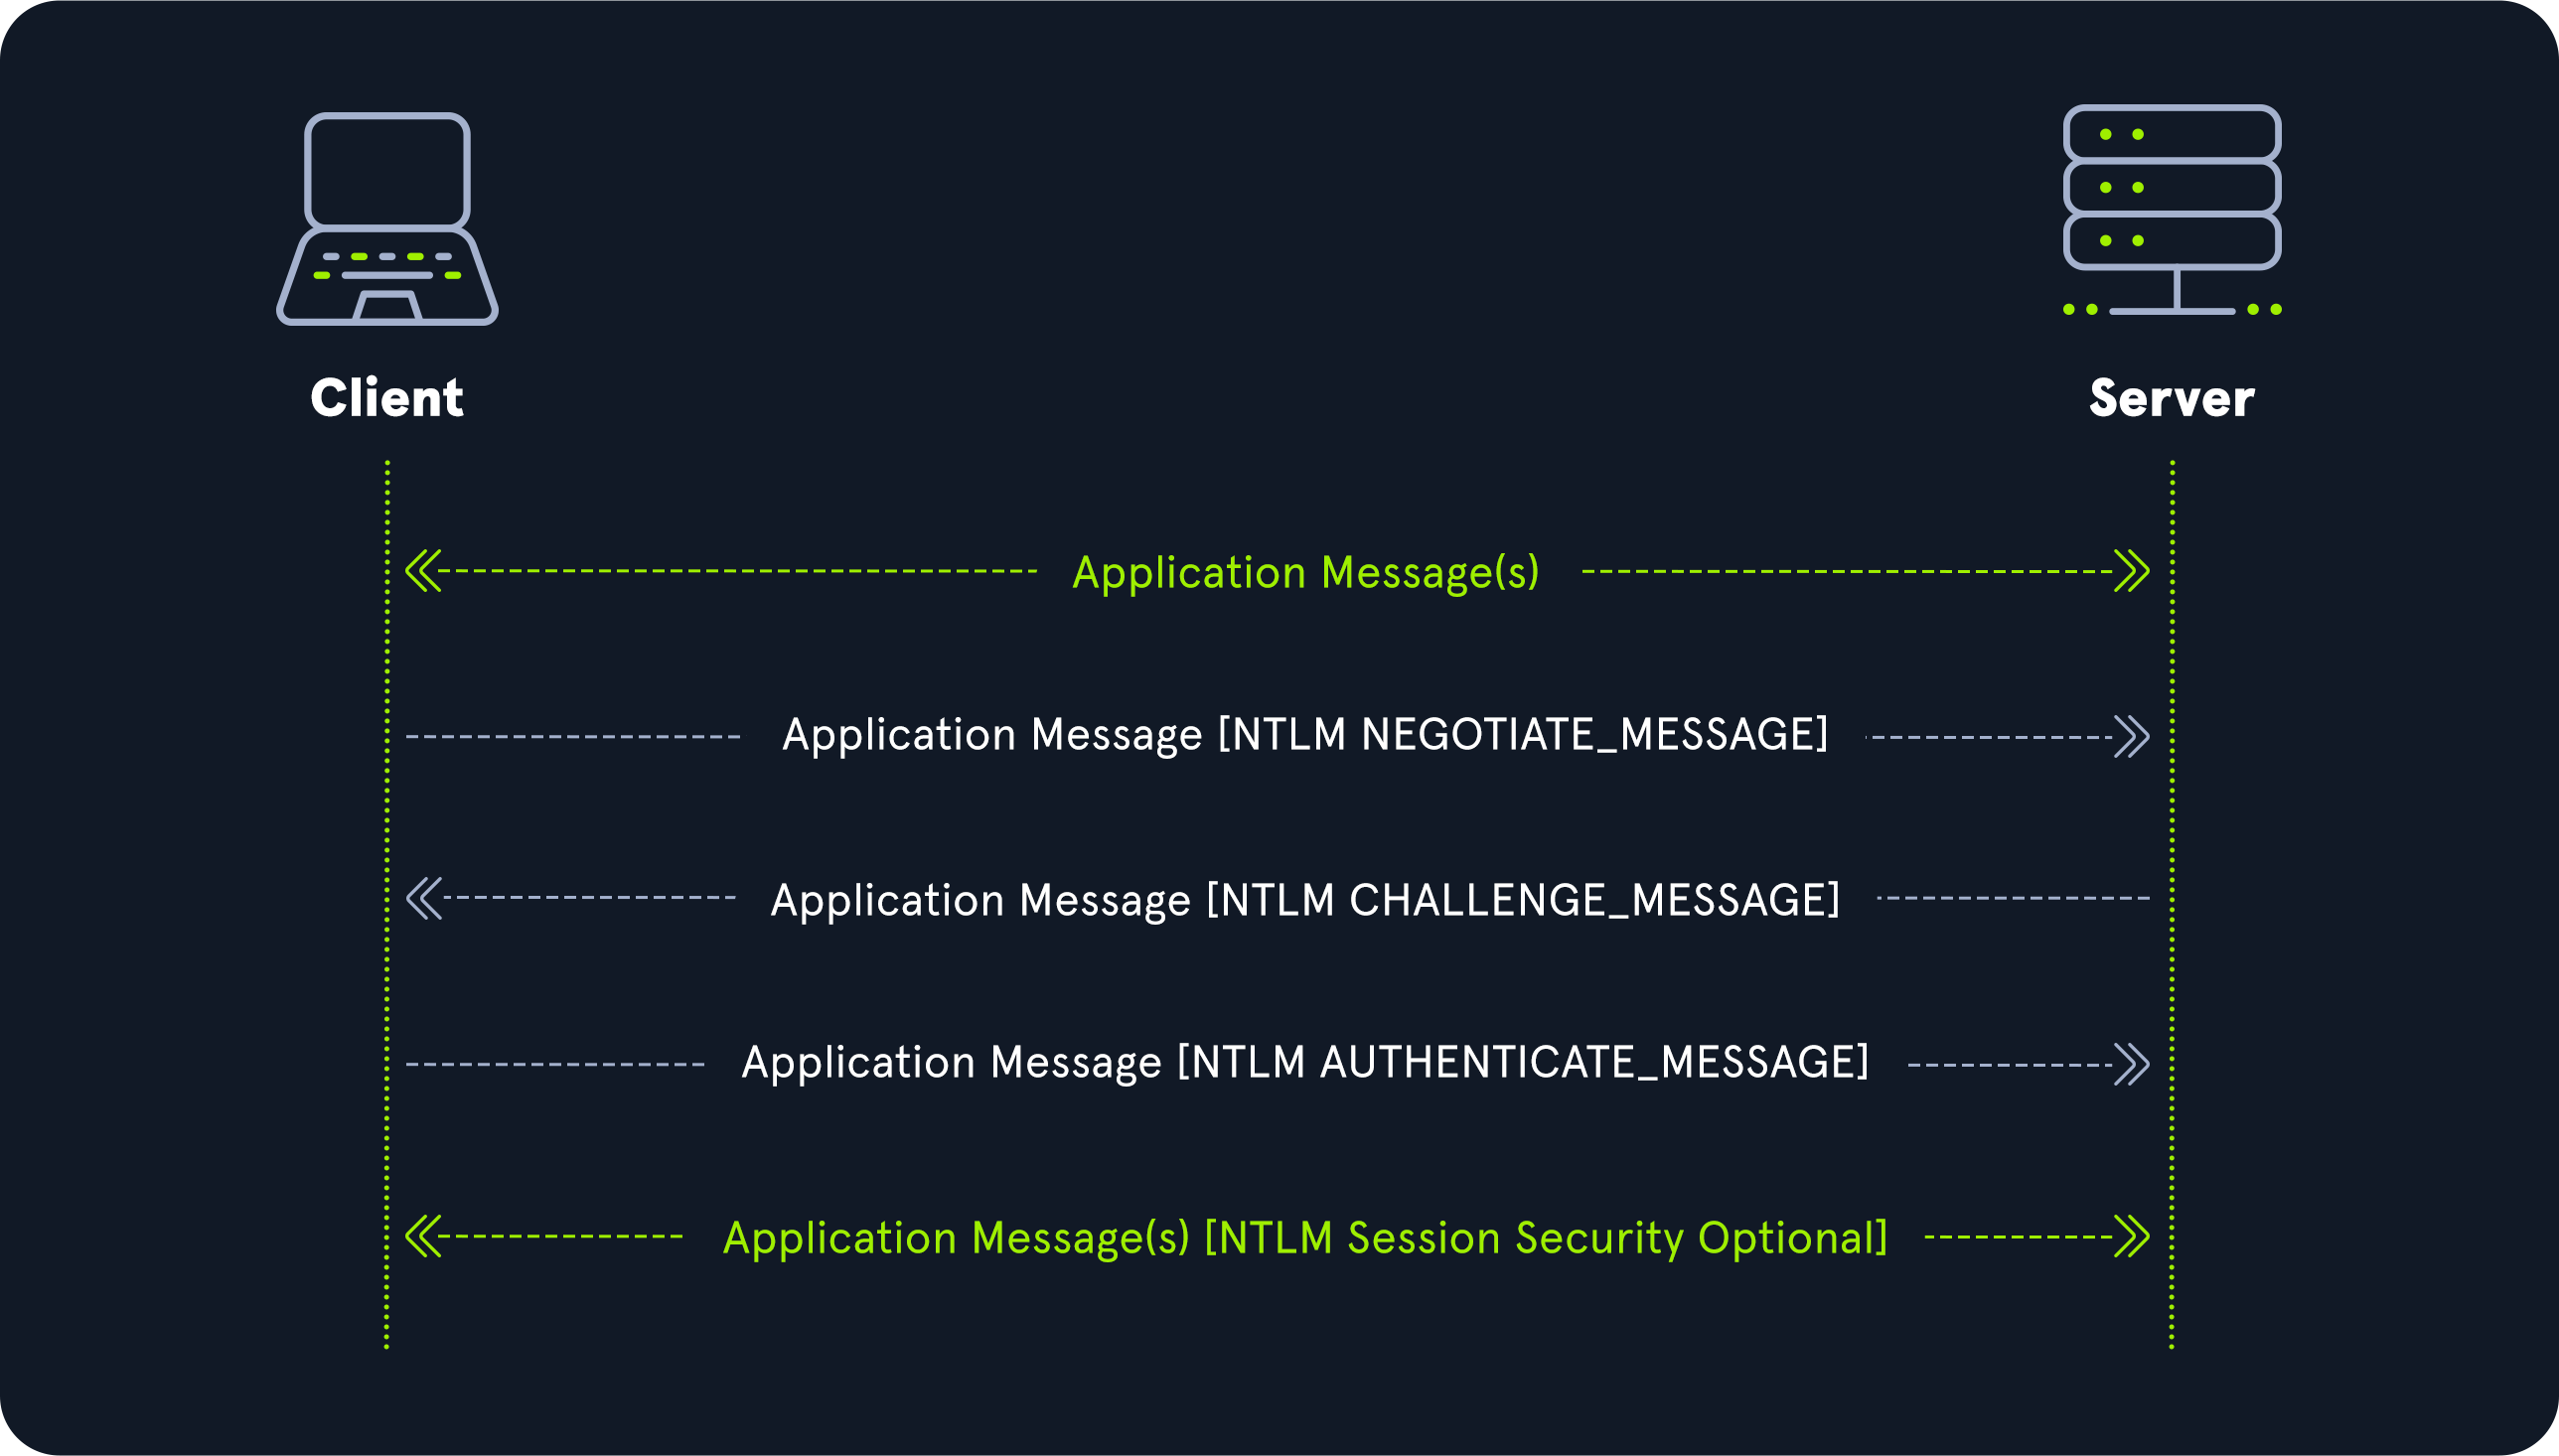
\includegraphics[width=\linewidth]{network/ntlm/images/Workgroup_Computers_NTLM_Authentication.png}
  \caption{Workgroup NTLM protocol}
  \label{fig:workgroup-ntlm-protocol}
\end{figure}

\subsubsection{NTLMv1 (Net-NTMLv1)}

The NTLM protocol performs a challenge/response between a server and  client using the NT hash. 

NTLMv1 uses both the NT and the LM hash, which can make it easier to "crack" offline after capturing a hash using a tool such as Responder or via an NTLM relay attack  

The protocol is used for network authentication, and the Net-NTLMv1 hash itself is created from a challenge/response algorithm. The server sends the client an 8-byte  random number (challenge), and the client returns a 24-byte response.  These hashes can NOT be used for pass-the-hash attacks. The algorithm  looks as follows:

\begin{verbatim}
C = 8-byte server challenge, random
K1 | K2 | K3 = LM/NT-hash | 5-bytes-0
response = DES(K1,C) | DES(K2,C) | DES(K3,C)
\end{verbatim}


\subsubsection{NTLMv2 (Net-NTLMv2)}
NTLMv2 provides three primary operations:
\begin{itemize}
    \item 
        Authentication.
    \item
        Message integrity, known as message signing in the NTLM terminology.
    \item 
        Message confidentiality, known as message sealing in the NTLM terminology.
\end{itemize}

NTLMv2 sends two responses to the 8-byte challenge received by the server.
These responses contain a 16-byte \verb+HMAC-MD5+ hash of the challenge, a
randomly generated challenge from the client, and an \verb+HMAC-MD5+ hash of the user's credentials. 

A  second response is sent, using a variable-length client challenge including the current time, an 8-byte random value, and the domain name.  

The algorithm is as follows:

\begin{verbatim}
SC = 8-byte server challenge, random
CC = 8-byte client challenge, random
CC* = (X, time, CC2, domain name)
v2-Hash = HMAC-MD5(NT-Hash, user name, domain name)
LMv2 = HMAC-MD5(v2-Hash, SC, CC)
NTv2 = HMAC-MD5(v2-Hash, SC, CC*)
response = LMv2 | CC | NTv2 | CC*
\end{verbatim}


We can see that developers improved upon v1 by making NTLMv2 harder to crack
and giving it a more robust algorithm made up of multiple stages. 

Here's an example of a Net-NTLMv2 (a.k.a NTLMv2) hash:
\begin{verbatim}
admin::N46iSNekpT:08ca45b7d7ea58ee:88dcbe4446168966a153a0064958dac6:5c7830315c78303100
00000000000b45c67103d07d7b95acd12ffa11230e0000000052920b85f78d013c31cdb3b92f5d765c783030
\end{verbatim}


\subsection{NTLM Session Security}

\subsubsection{Message Signing and Sealing}

\subsubsection{Extended Protection for Authentication (EPA)}



\subsection{Domain Cached Credentials (MSCache2)}
In an AD environment, the authentication methods mentioned in this  section and
the previous require the host we are trying to access to  communicate with the
"brains" of the network, the Domain Controller.  Microsoft developed the MS
Cache v1 and v2 algorithm (also known as Domain Cached Credentials  (DCC) to
solve the potential issue of a domain-joined host being unable  to communicate
with a domain controller (i.e., due to a network outage  or other technical
issue) and, hence, NTLM/Kerberos authentication not  working to access the host
in question. Hosts save the last ten hashes for any domain users that
successfully log into the machine in the
\verb+HKEY_LOCAL_MACHINE\SECURITY\Cache+  registry key. These hashes cannot be used in pass-the-hash attacks.  Furthermore, the hash is very slow to crack with a tool such as Hashcat,  even when using an extremely powerful GPU cracking rig, so attempts to  crack these hashes typically need to be extremely targeted or rely on a  very weak password in use. 

These hashes can be obtained by an attacker or pentester after gaining local
admin access to a host and have thefollowing format:
\begin{verbatim}
$DCC2$10240#bjones#e4e938d12fe5974dc42a90120bd9c90f
\end{verbatim}

